\begin{figure}[h]
    \centering
    
\includegraphics[width=0.5\textwidth]{pics/nest_js_logo.jpg}
    \caption{Nest.js Logo}
    \cite{Nest_js_logo}
    \label{fig:mesh1}
\end{figure}

Nest.js ist ein auf NodeJS basierendes Framework, welches Typescript und Vanilla JavaScript unterstützt. Es kombiniert Elemente von Object Oriented Programming, Functional Programming und Functional Reactive Programming. Im Hintergrund verwendet Nest.js, Express.js als robustes HTTP-Server Framework, dadurch verfügt Nest über eine gewisse Abstraktionsebene.
\cite{Nest_js_Introduction}

\subsubsection{Controllers}
Die Aufgabe eines Controllers besteht darin, requests der Applikation entgegenzunehmen und anschließend eine Response an den Client zurück zu liefern.

\begin{figure}[h]
    \centering
    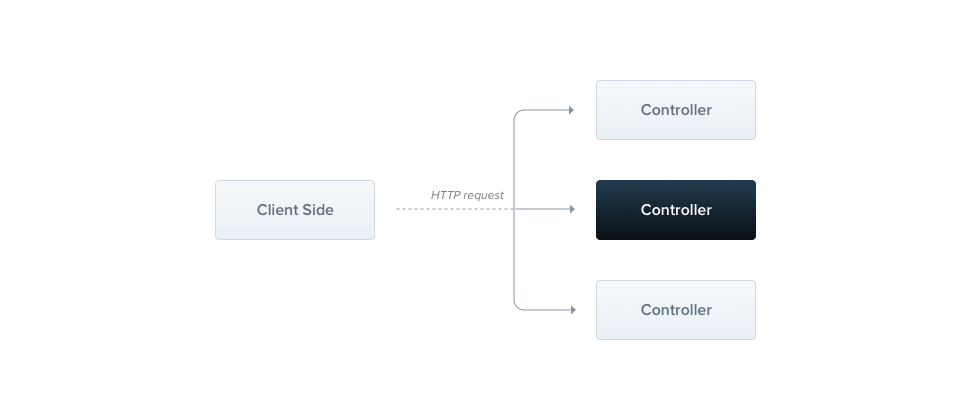
\includegraphics[width=1\textwidth]{pics/Nest_js_Controller.png}
    \caption{Nest.js Controller Architektur}
    \cite{Nest_js_Controller_Architektur}
    \label{fig:mesh1}
\end{figure}

Eingehende Requests werden durch den Routing Mechanismus an den zuständigen Controller weitergeleitet, welcher nun auf den Request reagieren kann und eine dementsprechende Response an den Client sendet. Um einen Controller zu erstellen, werden Klassen und Decorators benötigt. Decorators stellen erforderliche Metadaten, für die jeweiligen Klassen zur verfügung, dies ermöglicht es Nest, eine Routing-Map zu erstellen, um die Requests an die jeweilig zuständigen Controller weiterzuleiten.
\newline
Der @Controller Decorator ist nötig um einen neuen Basiscontroller zu erstellen. In diesem Decorator kann man einen Pfad Prefix definieren, um ähnliche Pfade leichter zu gruppieren und dadurch Codeverdoppelungen zu vermeiden. In der Klasse, welche mit dem Controller Decorator definiert wurde, kann man nun folgende HTTP-Methoden erstellen:

\begin{itemize}
    \item Get
    \item Post
    \item Put
    \item Delete
    \item Patch
    \item Options
    \item Head
    \item All
\end{itemize}

\vspace{5mm}

\begin{lstlisting}
import { Controller, Get } from '@nestjs/common';

@Controller('api/users')
export class UsersController {
    @Get(all)
    getAllUsers(): string {
        return 'This function returns all Users';
    }
}
\end{lstlisting}

Der oben gezeigte Beispielcode stellt einen vereinfachten Controller dar, welcher einen GET-Endpoint besitzt. Dieser gibt in folgendem Fall, den oben definierten String zurück.
\cite{Nest_js_Controllers}


\subsubsection{Vorteile}
\begin{itemize}
    \item Leistungsstark
    \newline
    Das Framework wurde so entwickelt, dass sich der Programmierer:in ausschließlich auf das Schreiben des Codes konzentrieren kann. Nest erledigt alle anderen Aspekte, wie zum Beispiel das Thema Sicherheit.
    \item Syntax
    \newline
    Die Syntax von Nest basiert auf dem Frontend Framework Angular, was es für Neulinge einfacher macht, sich in der Projektstruktur zurecht zu finden.
    \item Dokumentation
    \newline
    Die Dokumentation von Nest ist sehr detailliert und leicht zu verstehen.
    \item Typescript
    \newline
    Durch die Kompatibilität mit Typescript, verringert es die Fehleranfälligkeit des Codes, da man im Typescript Kompiliefehler und Warnungen angezeigt bekommt.
\end{itemize}

\subsubsection{Nachteile}
\begin{itemize}
    \item Kompliziert für Anfänger
    \newline
    Für Entwickler:innen die nicht mit Angular vertraut sind, kann das erlernen von Nest durchaus Schwierigkeiten mit sich bringen.
    \item Kein Know-How in Unternehmen
    \newline
    In Bezug auf diese Projektarbeit, ist einer der größten Nachteile für das Team, dass im Kooperationsunternehmen kein Know-How für Nest.js vorhanden ist, da dieses mit Express.js arbeitet.
\end{itemize}
\cite{Nest_js_Pros_Cons}
